\subsection{Q10.14 data 09202021 10082021 10312021 11092021 grouped by scenario \& x_first}

\begin{comment}
                     EFPR        EO      EFNR     n    pvalue
(frauth, False)  0.400000  0.600000  0.475000  40.0  0.184979
(frauth, True)   0.472222  0.527778  0.444444  36.0  0.764806
(icu, False)     0.424242  0.575758  0.545455  33.0  0.735384
(icu, True)      0.532258  0.467742  0.580645  31.0  0.657359
(rent, False)    0.283784  0.716216  0.445946  37.0  0.004610
(rent, True)     0.500000  0.500000  0.414286  35.0  0.899741
\end{comment}

\begin{table}[h]
    \centering
    \begin{tabular}{|c|c|c|c|c|c|c|}
        \hline
        scenario & x_first & EFPR & EO & EFNR & n & p-value\\
        \hline
        frauth & False & 0.400 & \textbf{0.600} & 0.475 & 40.0 & 0.185\\
		frauth & True & 0.472 & \textbf{0.528} & 0.444 & 36.0 & 0.765\\
		icu & False & 0.424 & \textbf{0.576} & \textbf{0.545} & 33.0 & 0.735\\
		icu & True & \textbf{0.532} & 0.468 & \textbf{0.581} & 31.0 & 0.657\\
		rent & False & 0.284 & \textbf{0.716} & 0.446 & 37.0 & \textbf{0.005}\\
		rent & True & 0.500 & 0.500 & 0.414 & 35.0 & 0.900\\
		
        \hline
    \end{tabular}
    \caption{Grouped by scenario x_first}
    \label{tab:my_label}
\end{table}
\begin{figure}[h]
    \centering
    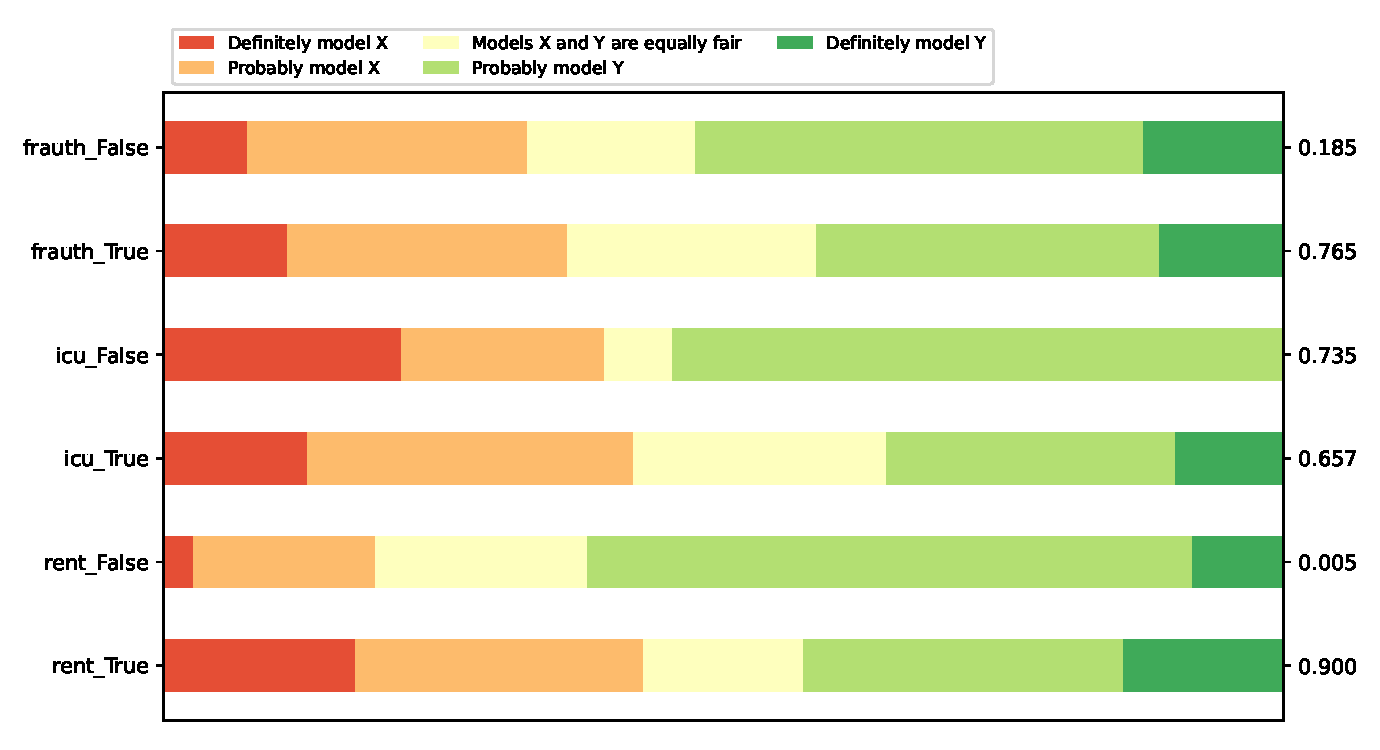
\includegraphics[width=0.8\textwidth]{figures/Q10.14/09202021_10082021_10312021_11092021/Q10.14_scenario_x_first.pdf}
    \caption{Grouped by scenario \& x_first}
    \label{fig:my_label}
\end{figure}
